\chapter{Introduction}

Scientists have spent decades building intricate mathematical models for systems and phenomena observed in all areas of life sciences. Such models have greatly expanded our understanding of the complex systems they describe, but the dramatic developments in technology and increase in widely available computational power in recent years have exposed another direction in which current research methodologies can progress.

Simulation in high performance computing environments is today the main approach used to validate scientific models in application domains ranging from astronomy to biomedical or earthquake science. Analytical solutions are often impossible to obtain, given the non-linear nature of these systems, so empirical observations drawn from running them in virtual settings is the only sensible option for further tuning and optimisation.

The prevalence of hypotheses developed by centralising and mining vast arrays of data sources has led to an era of data-centric research \cite{Goble2009}, where powerful cluster, grid and cloud computing platforms are open for scientific usage. However, the expertise required to operate this infrastructure is beyond the skill set of most researchers, so the efficiency of experimentation and the quality of insights drawn from it are heavily influenced by the performance of tools available to manage and process the available data.

\begin{figure}[h]
	\centering
		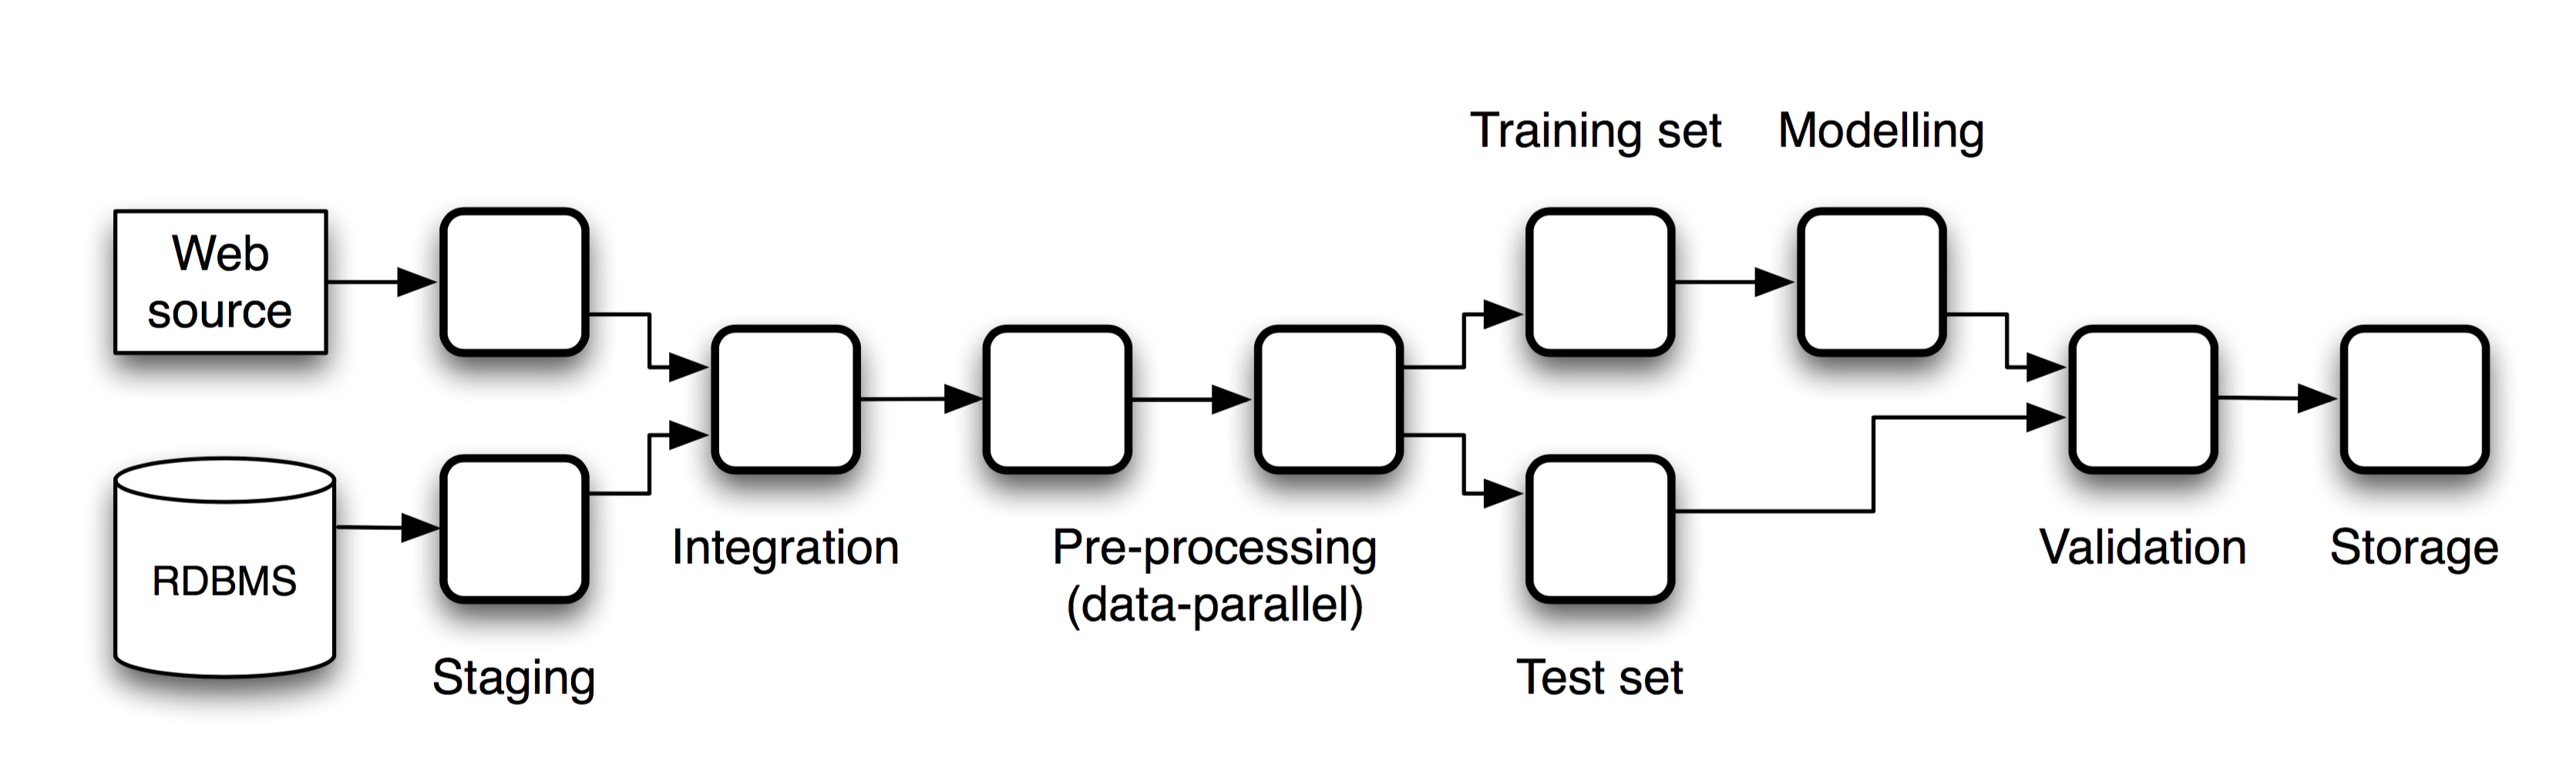
\includegraphics[scale=0.25]{WorkflowExample.png}
	\caption{Workflow example \cite{Curcin2008}.}
	\label{WorkflowExample}
\end{figure}

Workflow management systems provide support for creating data processing pipelines and automating historically tedious tasks such as tuning program parameters by running them repeatedly against many different datasets, defining work units and their interdependencies, or collecting and persisting results of analyses \cite{Goble2009, Taylor2007}. This is all achieved in the context of delegating the work efficiently over resources offered by distributed computing environments.

\section{Motivation}

Although multiple workflow management systems such as Taverna \cite{Taverna}, Kepler \cite{Kepler}, Pegasus \cite{Pegasus} or Galaxy \cite{Galaxy} are already established, many of them focus on specific scientific areas. Since the bioinformatics community is particularly active in adopting the usage of scientific workflows, tools like Galaxy and Kepler have been historically tailored for the needs of researchers in this field.

OpenMOLE \cite{Reuillon2013} is a scientific workflow engine that leverages the natural parallelism of simulation algorithms and targets distributed computing environments to run them. Compared to other existing platforms, OpenMOLE exposes some key features that make it unique:

\begin{itemize}
	\item It is not intended for use within a single scientific community, allowing for formalisms that make it generic.
	\item It focuses on hiding the complexity and heterogenity of hardware and software infrastructure that grids and clusters provide, separating the workflow definition from the underlying execution environment \cite{Reuillon2010}.
	\item By following a zero-deployment approach, it does not need any guarantees regarding the configuration of its runtime environment. It integrates a standalone packaging system, CARE \cite{Janin2014}, and it ensures reliable execution on remote hosts automatically by copying necessary resources on demand \cite{Reuillon2015}.
	\item It treats input models as black-boxes, allowing for interchangeable definitions in diverse languages or even packaged binaries \cite{Reuillon2013}. This means that already existing applications are not limited by a pre-configured toolbox and run as expected by default.
	\item The focus on flexible design and scalability generated control flow structures inexistent in most rival platforms. Some of these include loops, conditional branching, or the ability to include whole workflows as subtasks \cite{Reuillon2013}. This makes workflows reusable components that can be published and distributed on the OpenMOLE marketplace \cite{OpenMOLEMarketplace}.
	\item The DSL\footnote{Domain Specific Language} it uses to create workflows is an extension of the Scala \cite{Scala} programming language. This allows for type-safe job definitions and enables OpenMOLE to catch configuration errors earlier than other systems that rely on plain text descriptions.
\end{itemize}

Options that OpenMOLE currently offers to run workflows include:

\begin{itemize}
	\item Multithreading on a local machine.
	\item SSH connections to remote servers.
	\item Grids, such as EGI (European Grid Infrastructure) \cite{EGI}.
	\item Clusters managed by a wide range of software, including PBS\footnote{Portable Batch System} \cite{PBS}, Torque \cite{Torque}, SGE\footnote{Sun Grid Engine} \cite{SGE}, SLURM \cite{SLURM}, HTCondor \cite{HTCondor}, or OAR \cite{OAR}.
\end{itemize}

However, OpenMOLE does not support distributing the workload to cloud computing environments. at the moment. This is a significant disadvantage compared to other similar applications, since cloud providers are ubiquitous and cheap resources. Providing cloud support will enable a large user base to accelerate their research using OpenMOLE.

\section{Objectives}

The aim of this project is to enhance OpenMOLE by adding the ability to target computing clouds to the arsenal of available execution environments. More specifically, the main goal is to support running jobs on Amazon EC2\footnote{Amazon Elastic Compute Cloud} \cite{EC2}, while remaining generic enough to potentially integrate with other cloud providers and infrastructures (Google Cloud \cite{GoogleCloud}, OpenStack \cite{OpenStack} etc.), including Imperial College's Department of Computing private cloud that runs on a CloudStack \cite{CloudStack} deployment.

The key objectives of the project include:

\begin{itemize}
	\item Investigating the APIs\footnote{Application Programming Interface} and frameworks suitable to instantiate and coordinate computations on cloud infrastructures. In accordance with OpenMOLE's philosophy, we will favour Free and Open Source technologies. Initial steps involve researching the cloud distribution architecture of similar open source scientific workflow engines, as well as industrial software.
	\item Implementing a solution using the chosen tools as part of GridScale \cite{Passerat2016}, the engine powering OpenMOLE's distributed computation service. The library already has a modular structure, so development should be possible in isolation from the rest of the already production-ready modules.
	\item Fully automating the process of provisioning and and bootstrapping individual machines or clusters in the cloud. This should be invisible to the end user so that the only required configuration steps are entering the access credentials for the respective cloud and possibly setting up limits on resource consumption in order to avoid excessive costs.
	\item Evaluating the new environment against Amazon EC2, comparing its performance to benchmarks for already supported grids and clusters and, possibly, other workflow management systems. Comparison with other similar systems is considered a stretch goal, since the evaluation process would be tedious by requiring to define the work units for each system independently and results are likely to be spurious, since they might be caused by limitations in other parts of the system. Benchmarking performance between the cloud and a grid given the performance specifications of instances in both environments is expected to give more valuable results under these conditions.
\end{itemize}